\chapter{XLore系统与应用接口构建}
\label{cha:xlore-system-api}

\section{本章引论}
当前一些知名的知识库将自己的数据展示或发布出来,DBpedia[地址]提供最新的数据集下载、数据统计记录,甚至开源代码;Probase[地址]给出语义关系的数据集供研究人员使用,如is-a关系,同义词等。

中文知识库中,搜狗、百度等将知识图谱商业化,主要用来优化搜索、推荐实体等,百度用户通过搜索能获得图谱中相关实体的链接,但这些知识图谱只供自家公司商用,并没有开放数据。Zhishi.me作为第一个?科研领域的中文知识库,早期提供实体查询接口与SPARQL查询接口,现数据与网站都久未更新。

我们的中英文跨语言知识库XLORE,基于第三章跨语言知识库的数据,提供了数据展示页面、知识搜索功能、SPARQL查询接口、实例关系可视化、实体链接等多项功能,本章将具体阐述XLORE网站系统的搭建与数据接口的构建。

\section{XLore系统介绍}
XLORE网站系统旨在对外显示我们的数据数量与语义关系,并向用户提供便利的数据接口、清晰的数据展示。其对外网址为http://xlore.org。

截止到目前,XLORE网站提供三类知识展示与两种知识查询方式。

\subsection{XLore知识展示}
图\ref{fig:xlore-home}为XLORE网站首页。截止到2016年3月,我们的跨语言知识库中包含有xxx个概念、xxx个实例、xxx个属性。首页以表格的形式提供了顶层及其下两层的概念层及其统计数据,点击左边“+”按钮可获得子概念样例。除此之外,首页列出了一些实例例子,点击可直接查看相应实例页面。

\begin{figure}[H] 
  \centering
  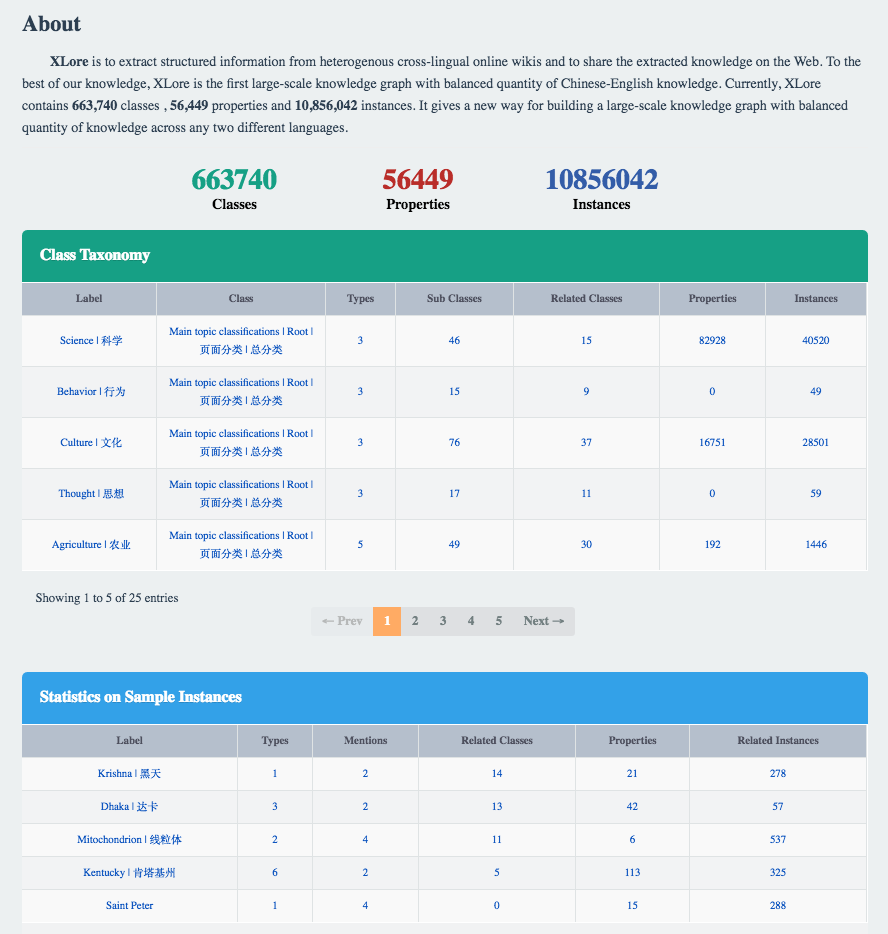
\includegraphics[width=0.8\columnwidth]{xlore-home}
  \caption{XLore网页系统首页}
  \label{fig:xlore-home}
\end{figure}

作为双语知识库,XLORE提供了语言切换功能,同时满足中文用户与外文用户的用户体验。

知识分为三种,分别为概念、属性、实例。概念页面以绿色为主色调,显示了概念中英文标签、父概念、子概念、相关实例等信息。属性页面使用紫色色调,展示了中英文标签、属性类型(Datetype与Objecttype)、相关实例、xx与xx等。

实例页面色调为蓝色,展示了中英文标签、实例图像、所属概念、摘要、信息框(包括中英文信息),URL多种信息。三种页面中,涉及到的双语内容,我们以“中文[英文]”的格式展示每条信息,如果网站语言为英文,则将英文展示在前,格式变为英文[中文]。当涉及到四个百科内容且无法融合,我们利用网页标签分栏的形式分别展示不同百科信息,如图\ref{fig:xlore-page}。

\begin{figure}[H] 
  \centering
  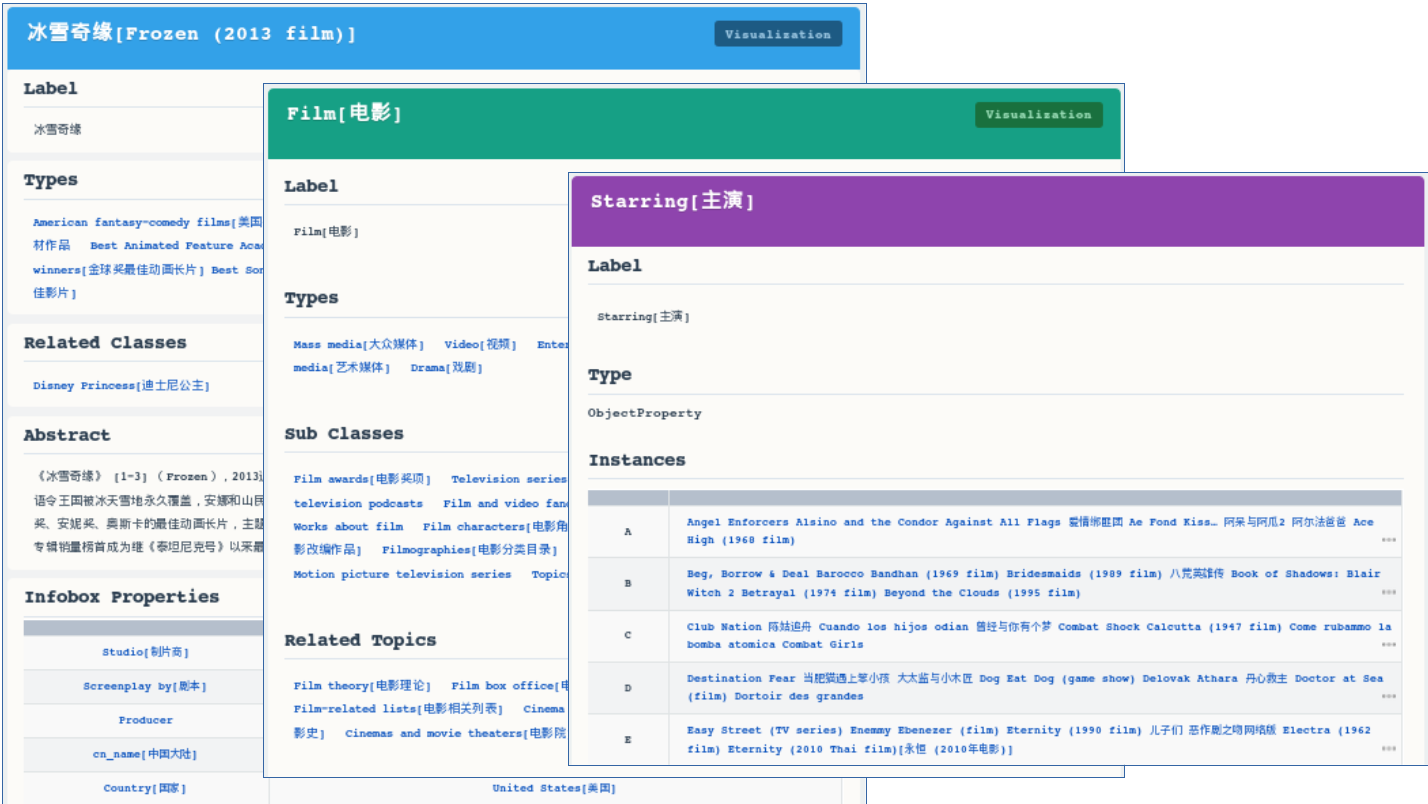
\includegraphics[width=1\columnwidth]{xlore-page}
  \caption{XLore实例、概念、属性页面展示}
  \label{fig:xlore-page}
\end{figure}

\subsection{XLore知识查询}
XLore提供搜索框文本查询与SPARQL语句查询。

搜索框在每个页面上都有,输入要查询的中文或英文字符串,点击“搜索”或按Enter键,即获得模糊查询结果。用户可根据需求选择搜索概念还是实例,或者属性,默认情况下,我们会同时返回三类搜素结果,用户可通过切换标签查看。图\ref{fig:xlore-search-engine}为搜索结果页面展示。

\begin{figure}[H] 
  \centering
  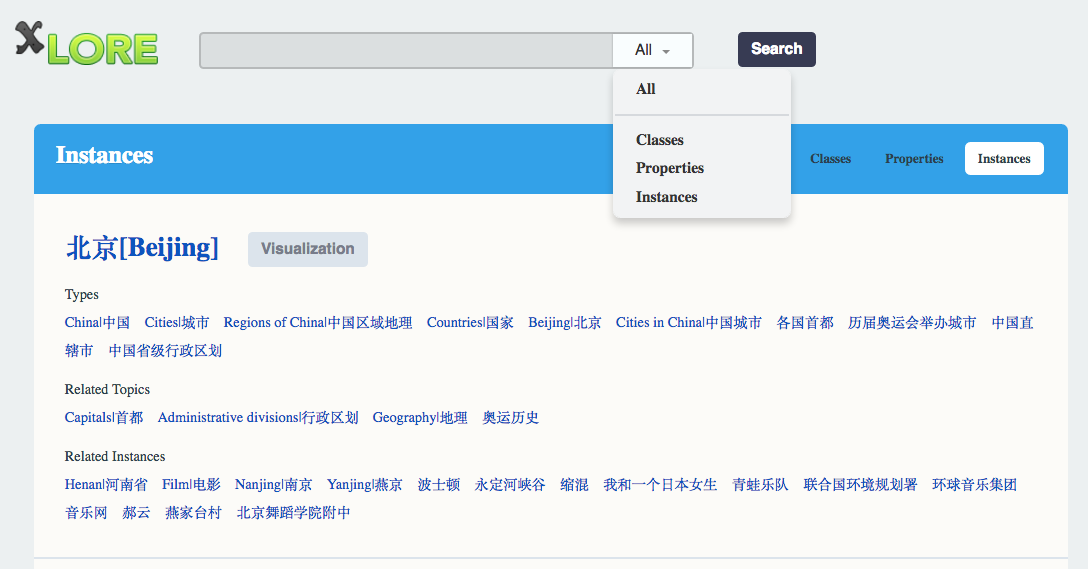
\includegraphics[width=0.9\columnwidth]{xlore-search-engine}
  \caption{XLore文本搜索框与搜索结果展示}
  \label{fig:xlore-search-engine}
\end{figure}

另一方面,对于专业人士,我们提供SPARQL查询页面,如图\ref{fig:xlore-sparql-endpoint}所示,输入正确的sparql语句,返回结果中可看到我们对知识库schema的定义。另外,为了防止sql注入造成的攻击与数据库崩溃,我们采取了xxx的安全措施。

\begin{figure}[H] 
  \centering
  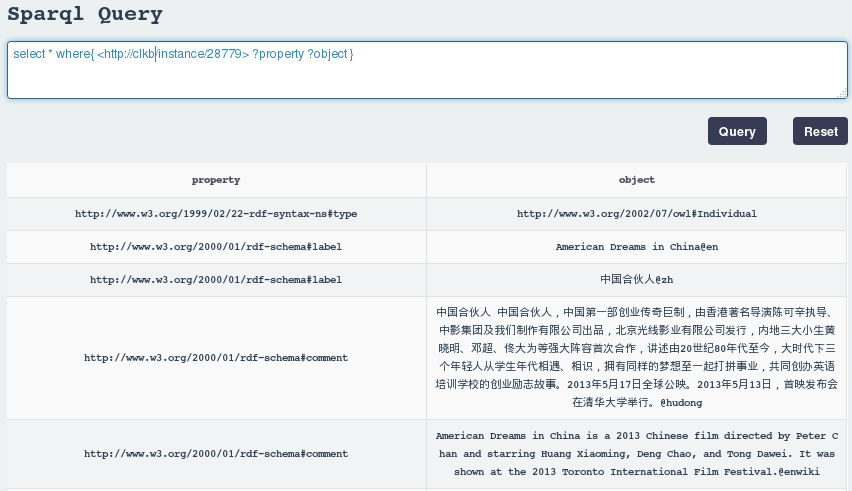
\includegraphics[width=0.9\columnwidth]{xlore-sparql-endpoint}
  \caption{XLore SPARQL 搜索框与搜索结果展示}
  \label{fig:xlore-sparql-endpoint}
\end{figure}

\subsection{XLore系统构建}
图xx为XLORE系统架构图。

xxx语义数据,我们的数据依托于图数据库。当前知名的的图数据库有Neo4J[引用],AllegroGraph[引用],Virtuoso等,鉴于我们的数据是以三元组的形式组织的,更适用于triple-store类型的数据库,因此我们选用商业版Virtuoso[网址](Virtuoso Universal Server)作为存储容器。

Virtuoso是由OpenLink软件公司开发的一个混合型数据库,它既支持传统的RDBMS数据,也支持RDF等其他图类型数据的存储与查询。其商业版本(Virtuoso Universal Server)可支持多CPU处理、多会话访问以及集群网络环境等。商业版Virtuoso是闭源的,但OpenLink公司提供一个名为OpenLink Virtuoso的开源版本[GitHub链接],供使用者编译与尝试。

为了提高搜索效率与召回率,我们对

Web框架采用JSP+Struts2.0搭建,运行在Tomcat7.0 Web服务器上。页面设计基于当前最受欢迎的Bootstrap前段框架。
对于概念与实例,我们基于D3.js可视化库[网址],提供了关系可视化,包括概念-子概念的关系,实例-相关实例的关系。图xx为可视化例子。

\section{XLore实体链接接口}

对同一个实体,外界有不同的称呼,比如演员xx,有昵称aa,bb,再比如电影yy,有名称dd,ee。另一方面,一个名称可能表征不同实体,比如xxxx。给出一个名称,在知识库中找出其对应的真正实体,被称作“实体链接”任务。如果我们能成功抽取出文本中的实体名称,并准确匹配出名称所代表的实体,对于该文本的理解有很大意义。Xxx任务中,xxxx(ji heng老师那个比赛),文章[][][]分别从xx,xxx,xx的数据集中,抽取出实体名称,提出相应的消歧算法,链接到xx知识库中。

XLORE作为一个通用领域的跨语言知识库,也提供了基于实体-名称词典扩展的实体链接接口。

XLORE实体链接接口提供了三种类型的查询:
1.  通用领域的名称查询:给出一个通用领域的名称,返回其在XLORE中最可能指向的一个或几个实体以及实体的中英文信息;
2.  通用领域的文本实体查询:给出一串文本,对文本进行实体名称抽取后,返回名称列表中各名称在XLORE中最可能指向的实体及实体的中英文信息;
3.  学术领域的名称查询:给出一个学术领域的名称,如“机器学习”,返回其在XLORE中学术领域指向的实体以及实体的中英文信息。

该接口框架图如下

具体来说,该接口以中英文名称或文本为输入,经过实体抽取、实体候选生成、实体消歧,确定与名称和上下文最匹配的实体,返回实体列表与中英文实体信息。


\subsection{实体抽取}
通用领域实体抽取使用xxx方法,主要获得xx,xxx,xxx类型的实体。
学术领域实体抽取采用xxx方法,该方法xxxx。

\subsection{实体候选生成}

实体候选从名称-实体词典中,通过名称获取相应的所有实体。其中,中英文名称-实体词典从中英文维基百科、百度百科、互动百科中抽取,选取以下几种元素构成:

1.  各百科的词条标题:百科中的每个词条都描述唯一实体,并维护着这个实体的相关信息。一般来说,词条标题是该实体公认的、最普遍的名称。对于无歧义的标题,记录其完整标题即可。然而,有些标题有多种含义。在百科中,如果一个标题有歧义,百科会通过在标题后加入分类信息来实现消歧,比如百度百科中,苹果(蔷薇科苹果属果实)代表一种水果,苹果(苹果产品公司)代表美国一家高科技公司,这种情况,标题“苹果”为实体“苹果(蔷薇科苹果属果实)”(在XLORE中有对应ID)的一个名称。

2.  各百科的文本内链接:百科词条的文本中,经常会有一些实体名称,以超链接的形式存在,指向该实体对应的词条。这个超链接的锚文本,可以看作是指向实体的同义词或别称,锚文本与实体词条构成一条名称-实体信息。

3.  各百科的消歧页面:如果一个名称可能对应多个实体,百科会为其创建一个歧义页面,供用户按所需选择词条。比如,“苹果”是一个歧义词汇,则歧义页面中会列举“苹果(蔷薇科苹果属果实)”、“苹果产品公司”等词条。维基百科通过“苹果\_(消歧义)”这样的页面[链接地址]展示词条,百度百科则通过为“苹果”父词条[链接地址]创建subview子词条来进行区分,如果一个词条没有歧义,则它的网页地址以id定位;如果一个词条有多种意思,则它的id页面为歧义页面,各子词条网址用subview id定位。消歧页面对于抽取实体的别称也有很大贡献。

4.  维基百科的重定向页面: 维基百科通过不断进行词条整理与更新,对一些陈旧的、非标准词条,或公认的缩写名称、别称等,将其自动定位到同一实体的标准词条页面上。原来的旧名称、缩写等可以看作实体的名称。比如中文维基中,“Microsoft”会被重定向到“微软”页面。

以2016年3月的中英文维基百科、2014年12月的百度百科、互动百科为数据源,我们获得名称-实体关系数量如表 \ref{tab:mention-entity}所示:

\begin{table}[htb]
  \centering
  \caption 名称-实体关系对抽取数量统计
  \label{tab:mention-entity}
  \begin{minipage}[t]{0.8\textwidth} % 如果想在表格中使用脚注,minipage是个不错的办法
    \begin{tabularx}{\linewidth}{l|X|X|X|X|}
      {\heiti } & {\heiti 英文维基} & {\heiti 中文维基} & {\heiti 百度百科} & {\heiti 互动百科} \\\midrule[1pt]
      标题 & 1 & 1 & 1 & 1 \\
      内链接 & 1 & 1 & 1 & 1 \\
      消歧页面 & 1 & 1 & 1 & 1 \\
      重定向页面 & 1 & 1 & 1 & 1 \\
      \bottomrule[1.5pt]
    \end{tabularx}
  \end{minipage}
\end{table}

最终获得中英文名称-实体对应关系总数量为:xxx对。
在抽取过程中,我们对名称-实体的出现频数进行了记录,用于之后的排歧工作,将会在xxx章详细说明。以”名称\\t实体知识库uri\\t该对出现频数”为格式存储数据,并以名称为索引,将数据导入到MySQL数据库中。

\subsection{实体消歧方法}
对于通用领域的名称查询,因为没有任何上下文信息,我们只能直接以频数从高到低排序,返回受认可的一个或多个实体信息。

对于通用领域的文本查询,我们根据上下文,为每个名称返回最相关的实体。具体来说:
\begin{itemize}
\item 1.  计算文本相关度:认为自身信息与上下文有关的实体更相关,提取实体上下文,与实体的摘要进行cosine相似度计算。
\item 2.  计算语义相关度:认为与文中其他实体有语义关系的实体更相关:提取根据文中其他实体,找出相关概念,xxxx。
\item 3.  取两个相关度的最大值。
\end{itemize}

对于学术领域的名称查询,我们利用知识库特有的领域限制,将实体的查找限制在相关概念下。

\subsection{实体链接接口的应用}
该实体链接接口的学术领域名称查找功能,应用在Aimer学术搜索系统[引用]的学术知识展示模块上,如图xx所示:用户在搜索学术领域词汇时,右边会显示该词汇对应的学术实体信息,及其相关上下文概念。

\section{本章小结}
本章对XLORE系统进行了详尽的介绍。为了进一步了解数据情况,我们搭建了网站展示XLORE知识,将数据直观地展现出来。同时,为了提高知识库的可用性,开发了实体链接接口,提供通用领域与指定领域的语义信息,也为下一步更精确的实体链接工作,做好铺垫。







